\documentclass{article}
\usepackage{graphicx}
\graphicspath{/}
\usepackage[utf8]{inputenc}

\title{Report on Application Execution times with Threading}
\author{Harsh Thakur}
\date{March 2018}

\begin{document}

\maketitle

\section{Scatter Plots}
Five different scatter plots are shown below each representing a thread configuration.
\begin{figure}[h]
    \centering
    \includegraphics{scatter_1}
    \caption{Plot of Execution time vs No. of Elements for $Thread\_1$ }
    \label{fig:Thread_1}
\end{figure}

The plot given in figure \ref{fig:Thread_1} gives execution time statistics when one thread is used.

\begin{figure}[h]
    \centering
    \includegraphics{scatter_2}
    \caption{Plot of Execution time vs No. of Elements for $Thread\_2$ }
    \label{fig:Thread_2}
\end{figure}

The plot given in figure \ref{fig:Thread_2} gives execution time statistics when two threads are used.

\begin{figure}[h]
    \centering
    \includegraphics{scatter_3}
    \caption{Plot of Execution time vs No. of Elements for $Thread\_4$ }
    \label{fig:Thread_4}
\end{figure}

The plot given in figure \ref{fig:Thread_4} gives execution time statistics when four threads are used.

\begin{figure}[h]
    \centering
    \includegraphics{scatter_4}
    \caption{Plot of Execution time vs No. of Elements for $Thread\_8$ }
    \label{fig:Thread_8}
\end{figure}

The plot given in figure \ref{fig:Thread_8} gives execution time statistics when eight threads are used.

\begin{figure}[h]
    \centering
    \includegraphics{scatter_5}
    \caption{Plot of Execution time vs No. of Elements for $Thread\_16$ }
    \label{fig:Thread_16}
\end{figure}

The plot given in figure \ref{fig:Thread_16} gives execution time statistics when sixteen threads are used.

\section{Line Plot}

\begin{figure}[h]
    \centering
    \includegraphics{line_plot}
    \caption{Plot of Avg. Execution time vs No. of Elements for all thread configurations }
    \label{fig:line_plot}
\end{figure}

The plot given in figure \ref{fig:line_plot} gives Average execution time statistics over 100 samples.

\section{Speedup Bar Graph Plot}

\begin{figure}[h]
    \centering
    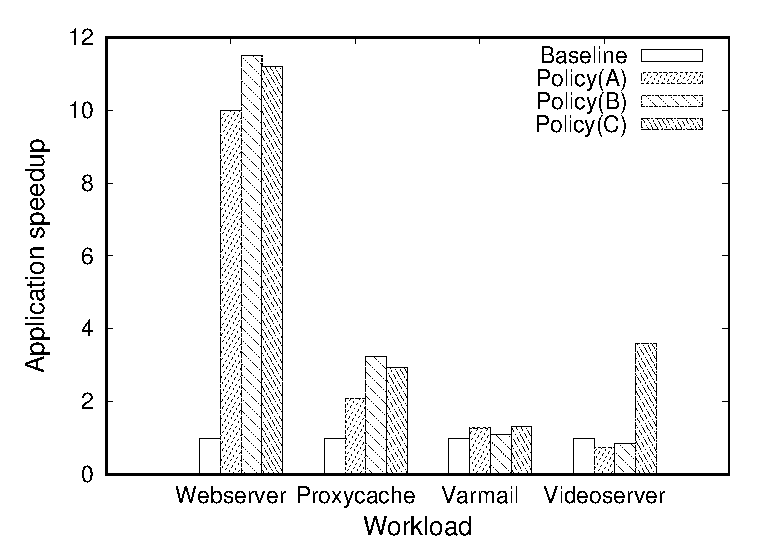
\includegraphics{speedup}
    \caption{Plot of Avg.Speedup vs No. of Elements for all thread configurations  }
    \label{fig:speedup_plot}
\end{figure}

The plot given in figure \ref{fig:speedup_plot} gives Average speedup statistics over 100 samples.

\section{Speedup Error Plot}

\begin{figure}[h]
    \centering
    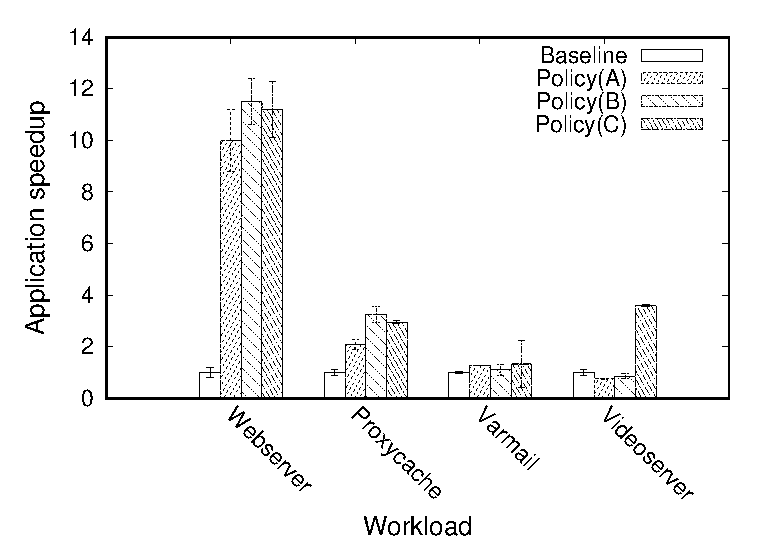
\includegraphics{speedup_errorbar}
    \caption{Plot of Speedup error vs No. of elements for all thread configurations }
    \label{fig:speedup_error}
\end{figure}

The plot given in figure \ref{fig:speedup_error} gives Speedup error (variance over 100 samples) statistics for all thread configurations.

\end{document}
